\newpage
\section{Análisis exploratorio de datos}

Para empezar con el entendimiento del data set decidimos hacer la siguiente división de las características:
\begin{itemize}
    \item Enfermedades
    \item Posibles causas
    \item Posibles consecuencias
\end{itemize}
Notar que esta división se basa en una hipótesis de cómo se relacionan los datos; más adelante veremos si la misma es acertada o si tiene errores.

\subsection{Indicadores sanitarios: Inmunización contra Hepatitis B, Polio y Difteria, y muertes infantiles por VIH/SIDA}
    \begin{itemize}
        \item Datos faltantes
        
            Se reportan $9$ datos faltantes en Hepatitis B.
            
        \item Tipo de datos
        
            Se observa que tanto Hepatitis B, Polio y Diphtheria cuantifican lo mismo (porcentaje de inmunización en menores de 1 año). Por lo tanto, comparar sus distribuciones será simple.
            Por otro lado, HIV/AIDS y Measles nos hablan de la cantidad de muertes entre 0-4 años cada 1.000 personas y los casos reportados cada 1.000 personas, respectivamente. Por otro lado, se ve que Measles no está reportando casos cada 1.000 habitantes como lo indica la consigna, por lo que decidimos descartarlos ya que no tenemos certeza de lo que representan.
        
        \item Distribución 
            
            Observemos la correlación entre las características previamente mencionados en la Figura \ref{fig:1}.
                        
            \begin{figure}[H]
            	\centering
            	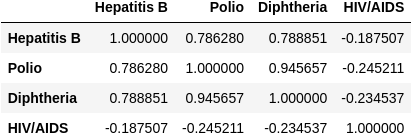
\includegraphics[width=0.35\textwidth]{img/1.png}
            	\caption{Matriz de correlación Hepatitis B, Polio, Diphtheria, HIV/AIDS.}
            	
            	\label{fig:1}
            \end{figure}
            
            Se ve una muy alta correlación entre Polio y Diphtheria y, a su vez, una considerablemente alta entre las mencionadas anteriormente y Hepatitis B. HIV/AIDS no tiene correlación con las demás, como esperábamos.
            
            
            Empecemos analizando las distribuciones de Hepatitis B, Polio y Diphtheria mediante un Boxplot que se ve en la Figura \ref{fig:2} y mediante histogramas como se ve en la Figura \ref{fig:3}.
            
             \begin{figure}[H]
            	\centering
            	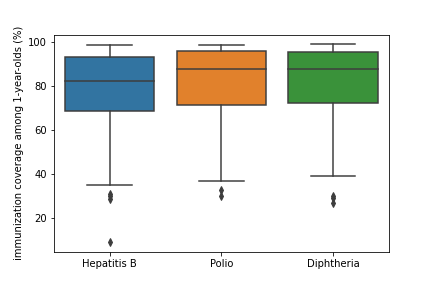
\includegraphics[width=0.35\textwidth]{img/2.png}
            	\caption{Boxplot Hepatitis B, Polio, Diphtheria.}
            	Se observan distribuciones muy parecidas en los tres casos.
            	\label{fig:2}
            \end{figure}
            
                    
               \begin{figure}[H]
              \centering
              \begin{subfigure}{0.3\linewidth}
                \centering
                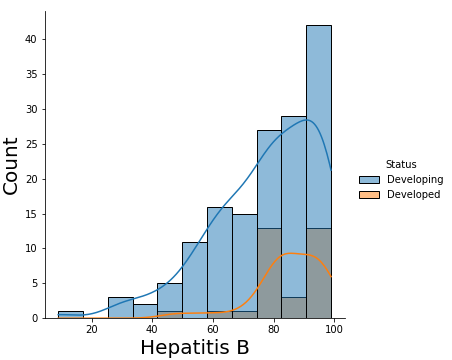
\includegraphics[width=\textwidth]{img/3.png}
              \end{subfigure}
              \hfill
                \begin{subfigure}{0.3\linewidth}
                \centering
                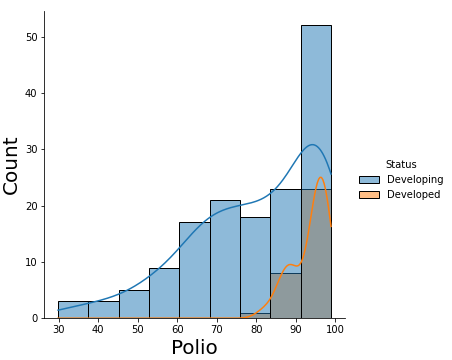
\includegraphics[width=\textwidth]{img/4.png}
              \end{subfigure}
                \hfill
                \begin{subfigure}{0.3\linewidth}
                \centering
                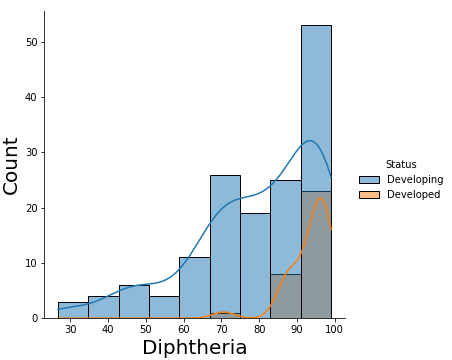
\includegraphics[width=\textwidth]{img/5.png}
              \end{subfigure}
               \caption{Histogramas Hepatitis B, Polio, Diphtheria.}
               \label{fig:3}
        \end{figure}

         En conclusión, Diphtheria, Polio y Hepatitis B tienen distribuciones muy similares y con una alta correlación, lo que nos permitiría unificarlas o descartar algunas de ellas de ser necesario.
         
         
         Se ve que en general, los países suelen tener un alto porcentaje de vacunados. Sin embargo, se ven casos atípicos en lo que esto no sucede; creemos que esto tendrá un impacto visible en la expectativa de vida.   
         
        Ahora, veamos el aspecto de la variable HIV/AIDS mediante un Boxplot e Histograma como se ve en la Figura \ref{fig: 4}.    
        
              
               \begin{figure}[H]
              \centering
              \begin{subfigure}{0.5\linewidth}
                \centering
               Tipo 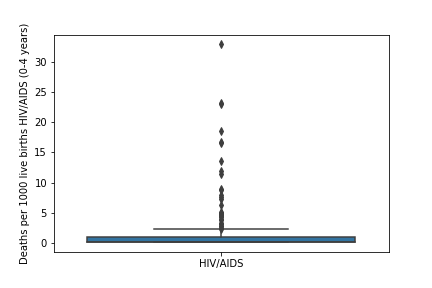
\includegraphics[width=\textwidth]{img/7.png}
              \end{subfigure}
              \hfill
                \begin{subfigure}{0.4\linewidth}
                \centering
                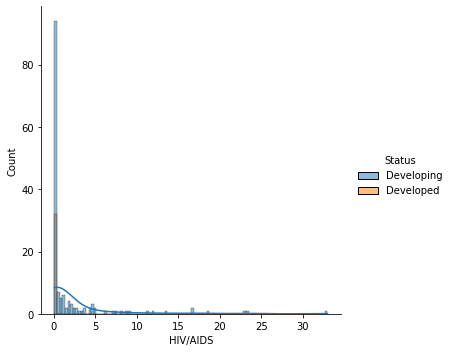
\includegraphics[width=\textwidth]{img/6.png}
              \end{subfigure}
               \caption{Distribución HIV/AIDS.}
               \label{fig: 4}
               
        \end{figure}
        
        Se ve que la mayoría de los países se concentran en alrededor de 0 a 5 muertes. Sin embargo, también podemos destacar la presencia de unos pocos outliers, que representan países con más casos, llegando a un máximo de alrededor de 30, los cuales creemos que tendrán un impacto en la expectativa de vida de estos países. Es notable que todos los países que tienen más de 5 muertes se encuentran en África. Esto podría explicarse en parte por la delicada situación económica de este continente, pero también por ser allí donde surgió esta enfermedad. 

       Veamos como se relaciona Life expectancy con estas variables, primero reportamos el coeficiente de correlación:
       
       \begin{verbatim}
            Hepatitis B        0.424982
            Polio              0.679231
            Diphtheria         0.672322
            HIV/AIDS          -0.587153
       \end{verbatim}
       
       Veamos mejor estas relaciones en la Figura \ref{fig: 5}. 
       
       
               \begin{figure}[H]
              \centering
              \begin{subfigure}{0.2\linewidth}
                \centering
                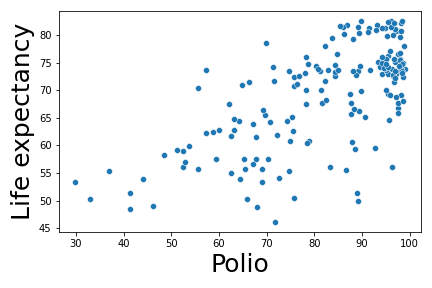
\includegraphics[width=\textwidth]{img/9.png}
              \end{subfigure}
              \hfill
                \begin{subfigure}{0.2\linewidth}
                \centering
                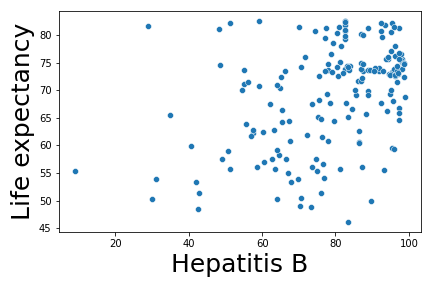
\includegraphics[width=\textwidth]{img/10.png}
              \end{subfigure}
              \hfill
                \begin{subfigure}{0.2\linewidth}
                \centering
                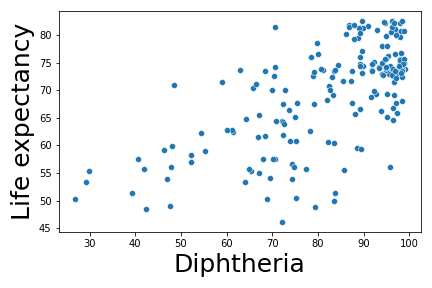
\includegraphics[width=\textwidth]{img/11.png}
              \end{subfigure}
                \hfill
                \begin{subfigure}{0.2\linewidth}
                \centering
                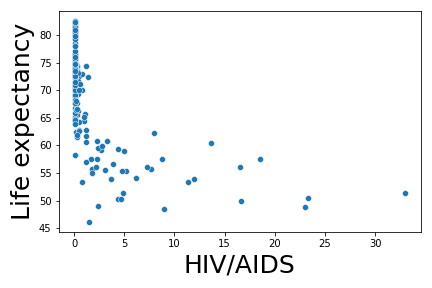
\includegraphics[width=\textwidth]{img/8.png}
              \end{subfigure}
               \caption{Scatterplot enfermedades VS Life expectancy.}
               	
               \label{fig: 5}
        \end{figure}
    \end{itemize}

Se ve que, como pensábamos, cuantos más vacunados hay, mayor es la expectativa de vida para las tres primeras y, cuantas más muertes se reportan, menor será la expectativa de vida en el caso de HIV/AIDS.

\subsection{Indicadores económicos: PBI, Composición del Ingreso, Gasto en Salud}
% Status	percentage expenditure	Total expenditure	GDP	Income composition of resources
    \begin{itemize}
        \item Datos faltantes
        
            Total expenditure tiene 2 NaNs, GDP 25 e Income composition of resources 10. Consideramos adecuado reemplazarlo por la mediana resultante para cada característica individual.
            
        \item Tipo de datos
        
            Status es una variable categórica, percentage expenditure en realidad no está reportando un porcentaje, encontramos valores mayores a 100, por lo que lo descartaremos.
            Total expenditure es un porcentaje, GDP es una variable numérica e Income composition of resources es otra variable numérica acotada del 0 al 1.  
            
        \item Distribución 
        
            Observemos la correlación entre las características previamente mencionados en la Figura \ref{fig: 6}.
            
              \begin{figure}[H]
            	\centering
            	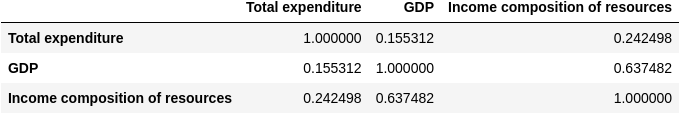
\includegraphics[width=0.50\textwidth]{img/12.png}
            	\caption{Matriz de correlación Total expenditure, GDP, Income composition of resources.}
            	No vemos una correlación muy significante entre ninguna de las características, aunque sí un poco más alta entre Income composition of resouces y GDP.
            	\label{fig: 6}
            \end{figure}
            
            Veamos si encontramos una relación entre las variables, más allá de la lineal, que nos ayude a interpretar nuestros datos en la siguiente Figura. 
            
               \begin{figure}[H]
              \centering
              \begin{subfigure}{0.3\linewidth}
                \centering
                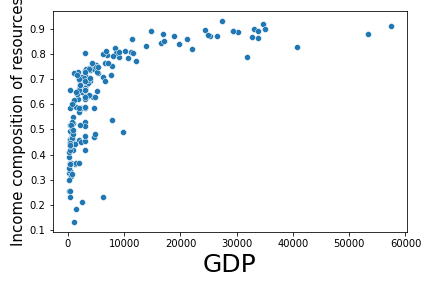
\includegraphics[width=\textwidth]{img/13.png}
              \end{subfigure}
              \hfill
                \begin{subfigure}{0.3\linewidth}
                \centering
                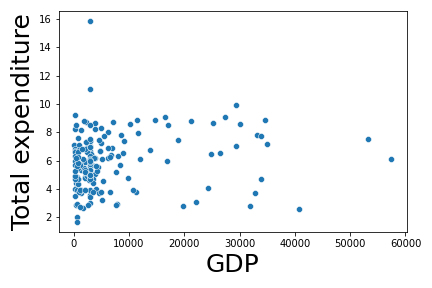
\includegraphics[width=\textwidth]{img/14.png}
              \end{subfigure}
                \hfill
                \begin{subfigure}{0.3\linewidth}
                \centering
                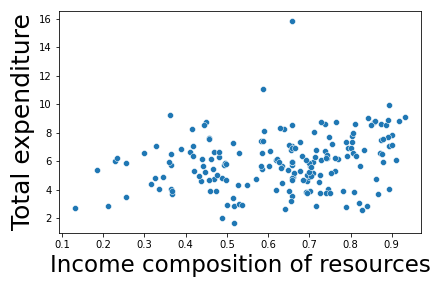
\includegraphics[width=\textwidth]{img/15.png}
              \end{subfigure}
               \caption{Scatterplots entre Total expenditure, GDP, Income composition of resources.}
               \label{fig: 7}

        \end{figure}

            En el primer gráfico se observa una relación particular entre GDP e Income composition of resources; si el GDP es muy bajo, el ICR puede tomar diversos valores, mientras que cuando el GDP es alto, el ICR también lo es, pero no podemos hablar de linealidad (se mantiene estático a partir de GDP = $20.000$ USD). Esto genera una curva de tipo exponencial.
            
            En el segundo y tercer gráfico no observamos nada que nos llame la atención, simplemente las variables están poco correlacionadas. Sin embargo, nos ayudan a entender las distribuciones de las variables; por ejemplo, podemos destacar que tanto Total expenditure como GDP tienen poca varianza, ya que vemos a todos los puntos concentrados en un espacio delimitado del gráfico b. De la misma manera se ve que ICR tiene mucha varianza.
            
            
            Para completar el análisis particular de estos datos, veamos sus respectivas distribuciones en la Figura \ref{fig: 8}.
            
            
                    
               \begin{figure}[H]
              \centering
              \begin{subfigure}{0.3\linewidth}
                \centering
                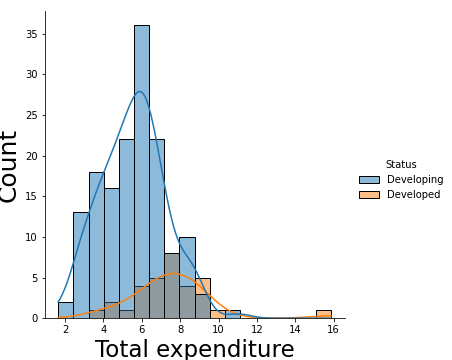
\includegraphics[width=\textwidth]{img/16.png}
              \end{subfigure}
              \hfill
                \begin{subfigure}{0.3\linewidth}
                \centering
                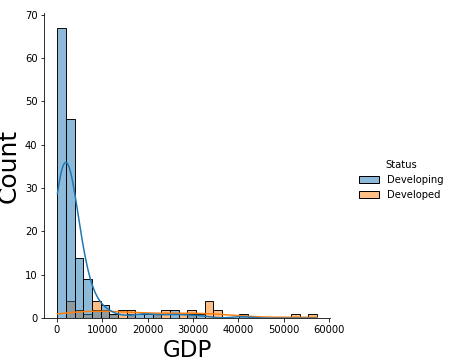
\includegraphics[width=\textwidth]{img/17.png}
              \end{subfigure}
                \hfill
                \begin{subfigure}{0.3\linewidth}
                \centering
                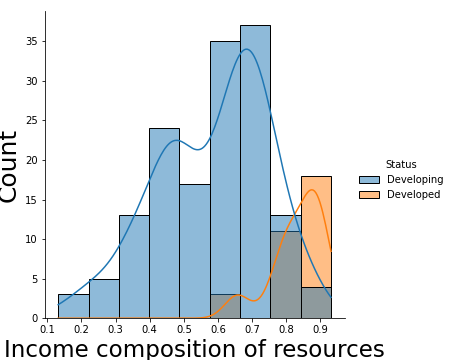
\includegraphics[width=\textwidth]{img/18.png}
              \end{subfigure}
               \caption{Histogramas Total expenditure, GDP, Income composition of resources.}
               \label{fig: 8}
        \end{figure}
            
            
            
            Tanto la distribución de Total expenditure como la de ICR tienen forma de campana de Gauss, con sus picos en 6 y 0.6, respectivamente. El GDP, por otro lado, tiene forma hiperboloide. Como es de esperar, los tres indicadores suelen ser mayores en los países 'desarrollados'. 
            
            Creemos que ICR estará correlacionada directamente con la expectativa de vida, ya que el bienestar económico influye de diversas maneras en la expectativa de vida, tanto a nivel individual como colectivo.
            
            Por la misma razón, esperamos que GDP correlacione positivamente con la expectativa de vida. Sin embargo, es posible que en menor manera, ya que el ICR es un índice más complejo que tiene en cuenta más factores, algunos relacionados con la distribución del ingreso. 
            
            Por otro lado, creemos que Total expenditure debería correlacionar positivamente, pero dudamos respecto a la magnitud. El hecho de que esté en términos absolutos, independientemente del nivel de población que tenga el país, lo hace un indicador poco informativo.
            
            Observemos los datos de la correlación a continuación y veamos si las hipótesis son ciertas:
            
             \begin{verbatim}
            Total expenditure                  0.288134
            GDP                                0.572807
            Income composition of resources    0.777659
       \end{verbatim}
       
       Veamos mejor estas relaciones en la Figura \ref{fig: 9}. 
       
       
               \begin{figure}[H]
              \centering
              \begin{subfigure}{0.3\linewidth}
                \centering
                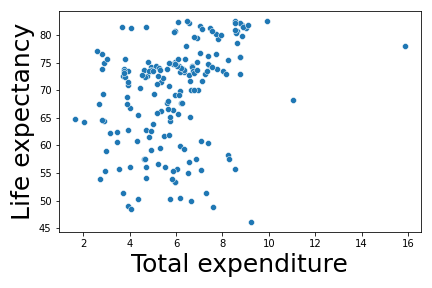
\includegraphics[width=\textwidth]{img/19.png}
              \end{subfigure}
              \hfill
                \begin{subfigure}{0.3\linewidth}
                \centering
                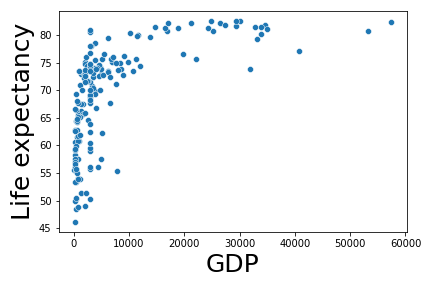
\includegraphics[width=\textwidth]{img/20.png}
              \end{subfigure}
              \hfill
                \begin{subfigure}{0.3\linewidth}
                \centering
                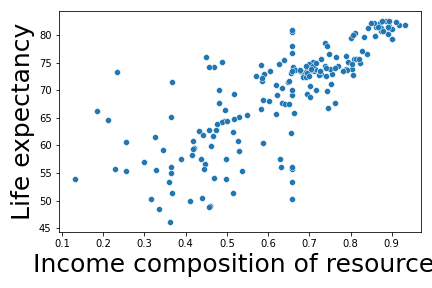
\includegraphics[width=\textwidth]{img/21.png}
              \end{subfigure}
               \caption{Scatterplot Life expectancy.}
               	
               \label{fig: 9}
        \end{figure}
  
    \end{itemize}
    
  Efectivamente podemos observar que prácticamente no existe correlación con Total expenditure. En cuanto a ICR y GDP, si bien tienen formas distintas, ambos cumplen una propiedad: un indicador alto garantiza una expectativa de vida alta, pero un indicador bajo no necesariamente implica lo contrario.  
  
\subsection{Indicadores Físicos: IMC, deladez entre 5-9 años y entre 1-19, consumo de Alcohol}   
% BMI, Alcohol   
\begin{itemize}
    \item Datos faltantes
    
    De BMI faltan dos. De alcohol falta uno. Estos campos serán completados utilizando la mediana de los mismos. De las variables thinness faltan dos en cada una.
    
    \item Tipo de datos
    
    Todas son variables numéricas. BMI es una métrica que relaciona el peso de un individuo con su altura ($\frac{peso}{altura^2}$). Los mismos están acotados. 
    
    Por otro lado, Alcohol representa el consumo \textit{per cápita} de alcohol puro en litros.
    
    Las variables thinness 5-9 y thinness 1-19 son un porcentaje.
    
    \item Distribución
    
    Calculamos el coeficiente de correlación entre estas variables y obtuvimos \texttt{0.504825}. 
    
    Para visualizar mejor la relación entre variables hacemos scatterplots (Figura \ref{fig: 10})
    
    \begin{figure}[H]
              \centering
              \begin{subfigure}{0.2\linewidth}
                \centering
                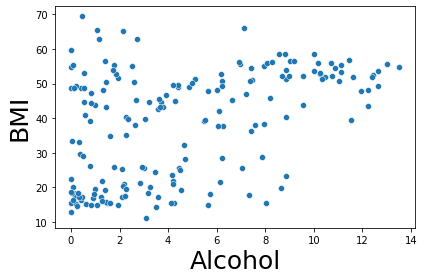
\includegraphics[width=\textwidth]{img/22.png}
              \end{subfigure}
              \hfill
                \begin{subfigure}{0.2\linewidth}
                \centering
                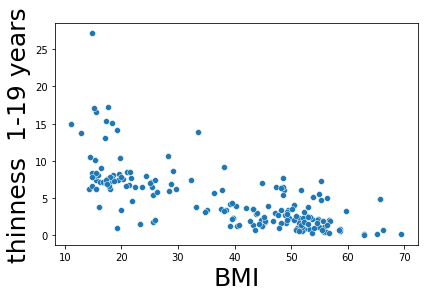
\includegraphics[width=\textwidth]{img/27.png}
              \end{subfigure}
                \hfill
                \begin{subfigure}{0.2\linewidth}
                \centering
                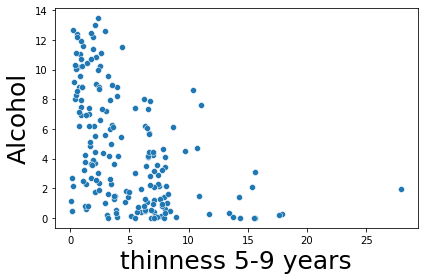
\includegraphics[width=\textwidth]{img/28.png}
              \end{subfigure}
                            \hfill
                \begin{subfigure}{0.2\linewidth}
                \centering
                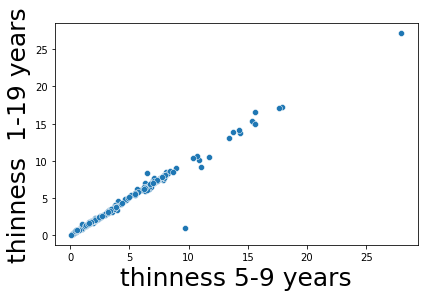
\includegraphics[width=\textwidth]{img/29.png}
              \end{subfigure}
               \caption{Scatterplots.}
               \label{fig: 10}
        \end{figure}
    
    En primer lugar, ambas variables thinness están fuertemente relacionadas, parecen prácticamente iguales. Esto tiene sentido, dado que indican lo mismo en distintas grupos demográficos, estando uno (5-9 años) incluido en el otro (1-19 años).  
    
    Por otro lado, vemos que BMI y thinness están inversamente relacionados; esto es porque lógicamente, un alto porcentaje de thinness implica un bajo BMI y viceversa.
    
    En cuanto a la característica alcohol, no se ve una correlación significante con ninguno de los demás.
    
    Ahora veamos la distribución de las mismas.
        
          \begin{figure}[H]
            \centering
              \begin{subfigure}{0.2\linewidth}
                \centering
                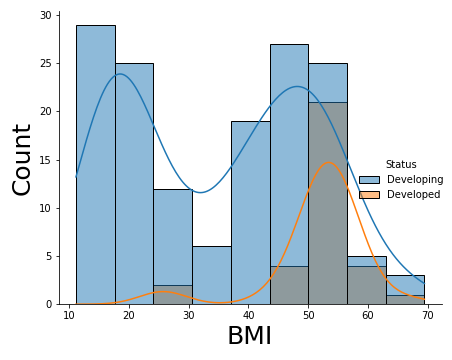
\includegraphics[width=\textwidth]{img/23.png}
              \end{subfigure}
              \hfill
                \begin{subfigure}{0.2\linewidth}
                \centering
                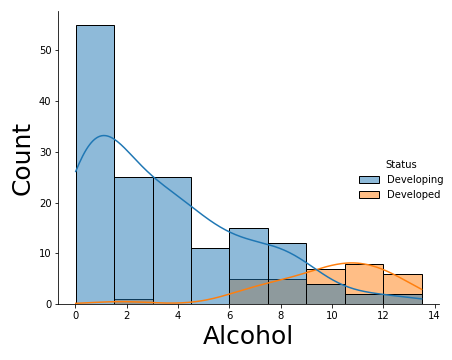
\includegraphics[width=\textwidth]{img/24.png}
              \end{subfigure}
              \hfill
                \begin{subfigure}{0.2\linewidth}
                \centering
                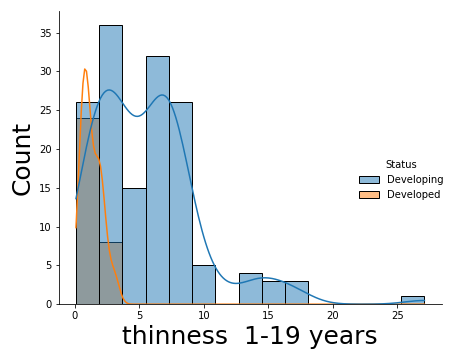
\includegraphics[width=\textwidth]{img/25.png}
              \end{subfigure}
                \hfill
                \begin{subfigure}{0.2\linewidth}
                \centering
                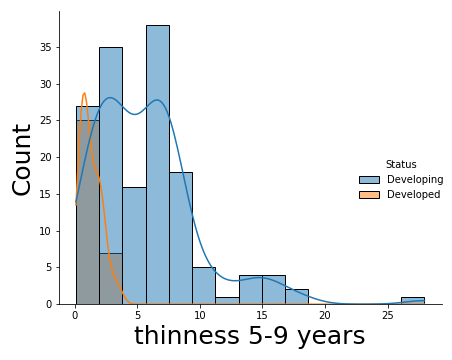
\includegraphics[width=\textwidth]{img/26.png}
              \end{subfigure}
               \caption{Distribución.}
               
               \label{fig: 17}
        \end{figure}
        
        BMI posee una distribución bimodal. Notemos que el BMI no debe tomar valores extremos, y que hay un intervalo óptimo en el cuál el coeficiente debería estar. Por lo tanto, creemos que la expectativa de vida sera más baja en países cuyo BMI se encuentre por encima (obesidad) o por debajo (desnutrición) de este intervalo. Creemos que los picos se corresponden con desnutrición y obesidad respectivamente. En países Developed el pico de desnutrición es muy bajo.
        
        En el gráfico de Alcohol podemos observar que en países Developing hay mucho menos consumo que en países Developed. Imaginamos que, a grandes rasgos, cuanto mayor sea el consumo de alcohol promedio, menor será la expectativa de vida, debido a los efectos del mismo sobre la salud.
        
        En cuanto a las variables de thinness, tal como se mencionó previamente, se ve la gran similitud entre ambas. Las mismas tienen, en países desarrollados, una gran concentración en valores cercanos a 0, y en países subdesarrollados hay dos picos: uno cercano a 0 y otro con valores más altos. Creemos que esto se debe a que dentro del grupo Developing entra una gran variedad de países con distintas realidades socio-económicas.
        
    Ahora veamos qué correlación tiene cada una de estas variables con Life expectancy.
    
          \begin{figure}[H]
            \centering
              \begin{subfigure}{0.2\linewidth}
                \centering
                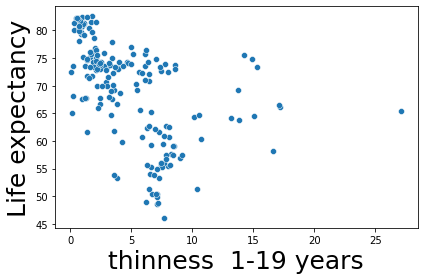
\includegraphics[width=\textwidth]{img/30.png}
              \end{subfigure}
              \hfill
                \begin{subfigure}{0.2\linewidth}
                \centering
                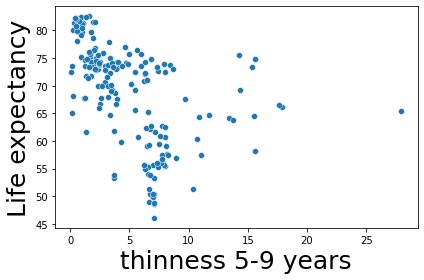
\includegraphics[width=\textwidth]{img/31.png}
              \end{subfigure}
              \hfill
                \begin{subfigure}{0.2\linewidth}
                \centering
                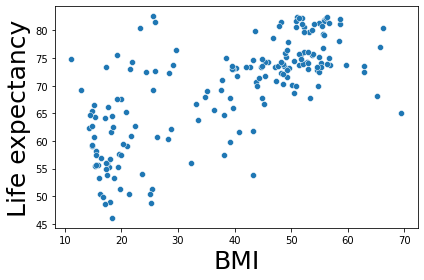
\includegraphics[width=\textwidth]{img/32.png}
              \end{subfigure}
                \hfill
                \begin{subfigure}{0.2\linewidth}
                \centering
                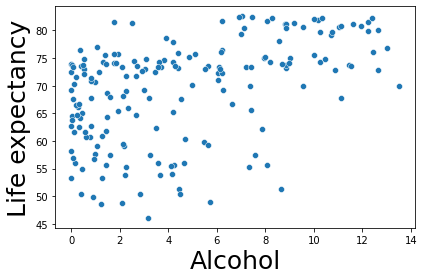
\includegraphics[width=\textwidth]{img/33.png}
              \end{subfigure}
               \caption{Scatterplots VS Life expectancy.}
               
               \label{fig: 18}
        \end{figure}    
    
    En los gráficos de las variables thinness (que son casi idénticos) se ve una relación inversa: a mayor thinness, menor Life expectancy. 
    Era esperable, dado que un bajo peso suele ser indicador de una nutrición precaria, lo que afecta gravemente a la salud (además de que la desnutrición puede entenderse como consecuencia de una situación socio-económica complicada, que también afecta a la expectativa de vida). 
    Resultados similares se observan con BMI.

    
    Alcohol presenta una leve correlación directa. Esto fue en contra de nuestras predicciones. Sin embargo, volviendo a observar los datos podemos entender que este efecto se puede deber a la correlación entre el consumo de alcohol y la riqueza de un país (en particular se observó que los países desarrollados consumen más alcohol que aquellos en vías de desarrollo).
    
    
    Veamos ahora los coeficientes de correlación obtenidos:
    
    \begin{verbatim}
   		
      thinness 1-19 years   -0.514356
      thinness 5-9 years    -0.507002
      BMI                   0.712117
      Alcohol               0.460338
    \end{verbatim}
    
    Entre éstas variables, la que presenta más correlación es BMI. 
\end{itemize}

%%%%%%%%%%%%%%%%%%%%%%%%%%%%%%%%%%%%%%%%%%%%%%%%%%%%%%%%    
    
\subsection{Otros indicadores: Mortalidad Adulta, Infantil, Escolarización y Población}

% Adult mortality: Adult Mortality Rates of both sexes (probability of dying between 15 and 60 years per 1000 population)

%- Infant deaths: Number of Infant Deaths per 1000 population

%- under-five deaths: Number of under-five deaths per 1000 population

%- Population: Population of the country

%- Schooling: Number of years of Schooling(years)



\begin{itemize}
    \item Datos faltantes
    
    De Population faltan 30 datos, y de Schooling faltan 10. Los reemplazamos por la mediana. El resto de las variables tiene todos sus datos presentes.
    
    \item Tipo de datos
    
    Todas son variables numéricas. Adult mortality, Infant deaths y under-five deaths representan cuántas muertes por cada 1000 personas ocurren según cada grupo etario.  Population es simplemente la población del país, y Schooling es la cantidad de años de escolaridad promedio.
    
    \item Distribución
    
    Para visualizar la correlación entre variables haremos scatterplots (Figura \ref{fig: 13})
    
    \begin{figure}[H]
              \centering
              \begin{subfigure}{0.15\linewidth}
                \centering
                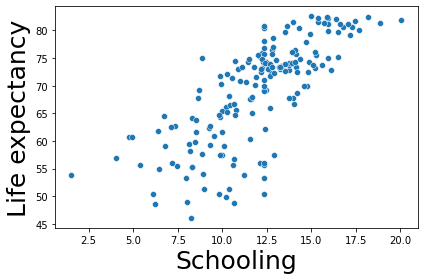
\includegraphics[width=\textwidth]{img/34.png}
              \end{subfigure}
              \hfill
                \begin{subfigure}{0.15\linewidth}
                \centering
                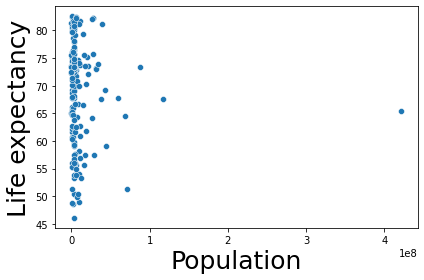
\includegraphics[width=\textwidth]{img/35.png}
              \end{subfigure}
                \hfill
                \begin{subfigure}{0.15\linewidth}
                \centering
                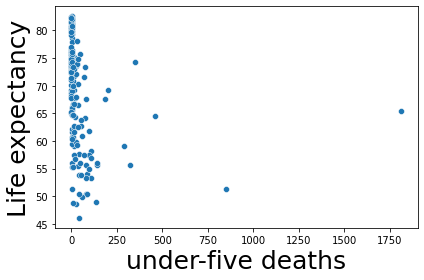
\includegraphics[width=\textwidth]{img/36.png}
              \end{subfigure}
                            \hfill
                \begin{subfigure}{0.15\linewidth}
                \centering
                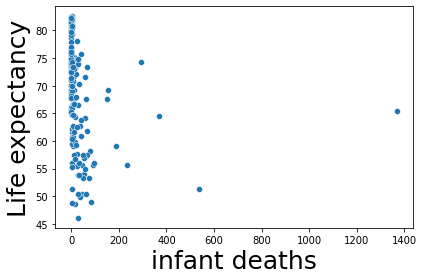
\includegraphics[width=\textwidth]{img/37.png}
              \end{subfigure}
                          \hfill
                \begin{subfigure}{0.15\linewidth}
                \centering
                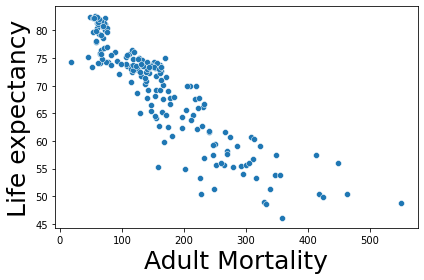
\includegraphics[width=\textwidth]{img/38.png}
              \end{subfigure}
               \caption{Scatterplots.}
               \label{fig: 13}
        \end{figure}

   Se ve una muy alta correlación con Schooling, lo que resulta lógico debido a que más años de educación parecerían indicar una mejor calidad de vida.
   
   Por otro lado, Population claramente no tiene ningún tipo de asociación con Life expectancy. 
   
   under-five deaths e infant deaths se comportan de una manera que no esperábamos; intuitivamente creeríamos que la mortalidad infantil esta muy correlacionada con la expectativa de vida. Sin embargo, eso no está sucediendo con nuestros datos; nos damos cuenta de que la razón de esto es porque los datos parecen estar mal.
   
   Se ven datos mayores a 1750 muertes cada 1000 habitantes, lo que no tiene sentido y nos lleva a descartar ambas características. Aunque reportar este error antes nos hubiese ahorrado algo de tiempo, nos damos cuenta del poder de un data-explore.
   
   
    Ahora veamos la distribución de Schooling, Population y Adult Mortality.
        
          \begin{figure}[H]
            \centering
              \begin{subfigure}{0.3\linewidth}
                \centering
                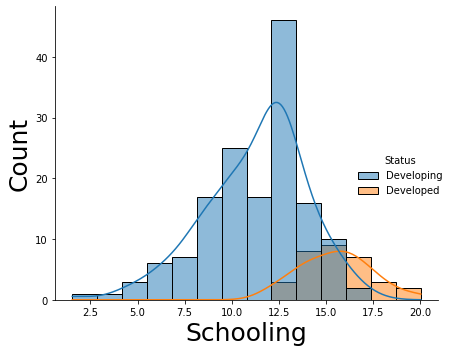
\includegraphics[width=\textwidth]{img/39.png}
              \end{subfigure}
              \hfill
                \begin{subfigure}{0.3\linewidth}
                \centering
                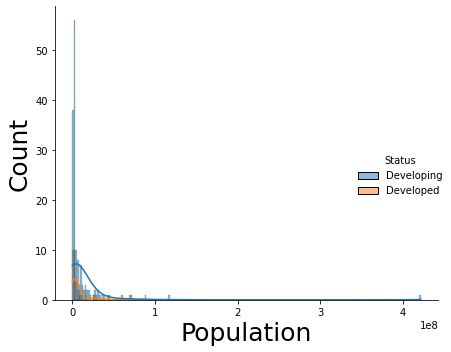
\includegraphics[width=\textwidth]{img/40.png}
              \end{subfigure}
              \hfill
                \begin{subfigure}{0.3\linewidth}
                \centering
                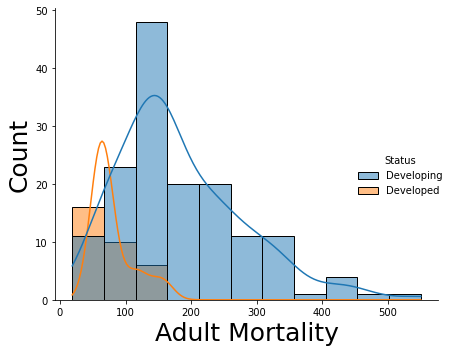
\includegraphics[width=\textwidth]{img/41.png}
              \end{subfigure}
               \caption{Distribución.}
               
               \label{fig: 17}
        \end{figure}
        
Tanto para Schooling y Adult Mortality se observan curvas normales y para los países desarrollados se observa más cantidad de años escolares y menos mortalidad en adultos que para los sub-desarrollados. 
 
En cuanto a Population, se observa una curva esperable. Sin embargo, no creemos que este dato nos sea de mucha utilidad.        
     
\end{itemize}    
    
    
    
% Podría hacerse mientras se hace sección 6. \subsubsection{Relación entre enfermedades, causas y consecuencias}
   